
% \begin{frame}{ Understand disorders of dynamics }
%     \begin{itemize}
%         \item
%     \end{itemize}{}
% \end{frame}{}

% \begin{frame}{Behavior is contrived and frequently doesn't generalize}
%     \begin{itemize}
%         \item
%     \end{itemize}{}
% \end{frame}{}

% \begin{frame}{Attractors suggest that synthetic states -> plausible states (meh}
%     \begin{itemize}
%         \item
%     \end{itemize}{}
% \end{frame}{}



\begin{frame}{Goals}
The main goals for this slide:
\begin{itemize}
	\item This is just to show you how this \empy{template} works
	\item There are two `emphasize' functions used to highlight \& italicize texts
	\begin{itemize}
		\item `\textbackslash empy' does \empy{this} and `\textbackslash empr' does \empr{this}.
	\end{itemize}
	\item The colors in this template is selected from the official Stanford Identity website: \href{https://identity.stanford.edu/color.html}{https://identity.stanford.edu/color.html}
	\item Note that hyperlinks, by default, are not highlighted. Of course, you can change this: e.g., \empr{\href{https://github.com/sanhacheong/stanford_beamer_presentation}{https://github.com/sanhacheong/stanford\_beamer\_presentation}}
\end{itemize}
\end{frame}



\begin{frame}{Example}
A (hopefully) useful function in this \LaTeX~template is:
\begin{center}
	\textbackslash examplebox\{ExampleTitle\}\{ExampleContents\}
\end{center}
which does this:
\examplebox{Example of the Command \textbackslash examplebox}{
This is what it does. Pretty self-explanatory, isn't it?

Given the color them, I \empr{recommend} using \textbackslash empr inside of examplebox. The \textbackslash empy command does not look \empy{that} good.
}
\end{frame}



\begin{frame}{References}
\begin{thebibliography}{3}
	\bibitem{myself}
	S.~Cheong. \empr{\href{https://github.com/sanhacheong/stanford_beamer_template}{https://github.com/sanhacheong/stanford\_beamer\_presentation}}. {GitHub}, August 2017.
\end{thebibliography}
\end{frame}


\begin{frame}{ Canonical circuits }
    \centering
    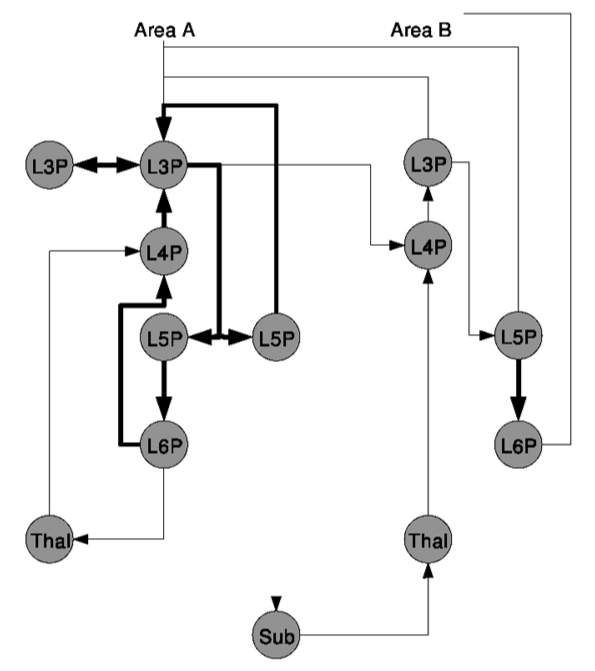
\includegraphics[height=0.8\textheight]{media/canonical}\nakedfootnote{Douglas \& Martin, 2004.}
\end{frame}
%
% \begin{frame}{ Functional motif discovery via optogenetics}
%     \begin{center}
%         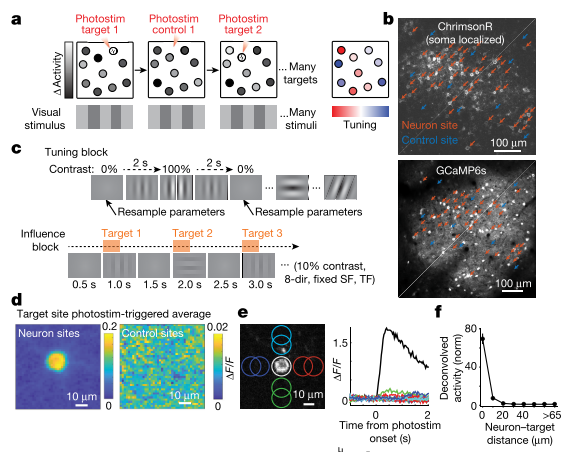
\includegraphics[height=0.85\textheight]{media/chettih_v1.png}
%         \,
%         Photostimulation-triggered average fluorescence changes.
%         \nakedfootnote{Selmann Chettih \& Christopher Harvey \emph{Nature}. 2019}
%     \end{center}
%     \note{\textbf{Placeholder}: TODO replace with fig showing competition vs mixed network (Fig 5?)}
% \end{frame}{}
